\documentclass[presentation,aspectratio=169]{beamer}

\usecolortheme{Imperial}
\setbeamertemplate{navigation symbols}{}
\setbeamertemplate{caption}[numbered]

\usepackage[utf8]{inputenc}
\usepackage[brazil]{babel}
\usepackage{booktabs}
\usepackage{caption}
\usepackage{graphicx}
\usepackage{amsmath}
\usepackage{amsfonts}
\usepackage{amssymb}
\usepackage{datetime}
\usepackage{icomma}
\usepackage{multirow}
\usepackage{multicol}
\usepackage{xcolor}
\usepackage[caption=true,font=footnotesize]{subfig}
\usepackage{siunitx}
\sisetup{output-decimal-marker = {,}, group-minimum-digits=3, group-separator={.},binary-units=true}

\definecolor{cinza}{rgb}{0.95, 0.95, 0.95}
\definecolor{alerta}{RGB}{0,129,208}
\setbeamercolor{alerted text}{fg=alerta}
\setbeamercolor*{item}{fg=alerta}
\setbeamercolor{block body}{fg=black,bg=cinza}
\setbeamercolor{block title}{bg=alerta!60!white,fg=white}
\setbeamertemplate{blocks}[rounded][shadow=true]

\setbeamertemplate{footline}[text line]{%
  \parbox{\linewidth}{\vspace*{-8pt}\textcolor{imperialblue}{Jesus Dourado de Albuquerque (jda.eng17@uea.edu.br)\hfill\insertpagenumber/\inserttotalframenumber}}}

% -----------------------------------------------------------------------------
\AtBeginSubsection[]
{
  \begin{frame}[plain]{Outline}
   \tableofcontents[
    sectionstyle=show/shaded,
    subsectionstyle=show/shaded,
    ]
  \end{frame}
}

\AtBeginSection[]
{
  \begin{frame}[plain]{Agenda}
   \tableofcontents[
    sectionstyle=show/shaded,
    subsectionstyle=show/shaded,
    ]
  \end{frame}
}

%Information to be included in the title page:
\title{\LARGE{Uma aplicação de Redes Neurais Convolucionais Regionais para Detecção de Malária}
}

\author{\textbf{Jesus Dourado de Albuquerque}\\
\textbf{Orientadora}:  Prof. Dra. Elloá Barreto Guedes da Costa\\
\footnotesize{\emph{\{jda.eng17, ebgcosta\}@uea.edu.br}}\\
\small{\emph{\textcolor{imperialblue}{Trabalho de Conclusão de Curso 2022}}}
}

\institute{\small{Laboratório de Sistemas Inteligentes\\
Escola Superior de Tecnologia\\
Universidade do Estado do Amazonas}
}

\date{}

\begin{document}

{
\setbeamertemplate{footline}{}
\frame{\titlepage}
}

\institute{}


\section{Introdução}
%!TEX root=../main.tex

\begin{frame}{Motivação e Contextualização}
\begin{itemize}
    \item A malária é uma doença causada pelo protozoário do gênero \emph{Plasmodium}, transmitida pelo mosquito do gênero \emph{Anopheles} \cite{OMS:Malaria2019}
    \ \ \newline
    \item A enfermidade é um problema grave de saúde, sendo uma das principais doenças letais em regiões tropicais \cite{OMS:Malaria2019}
    \ \ \newline
    \item Segundo a OMS, foram registrados 228 milhões de casos e 405 mil mortes em âmbito global, a grande maioria ocorreu na África 
     \ \ \newline
    \item O Brasil, no anos de 2020 e 2021, registrou 141 mil e 135 mil casos, respectivamente \cite{Boletim:Malaria2022}
\end{itemize}
\end{frame}

\begin{frame}{Motivação e Contextualização}
    \begin{itemize}
        \item O diagnóstico precoce é importante para o tratamento adequado \cite{Berzosa:MalariaDiagnostico}
        \ \ \newline
        \item  Existem 2 tipos de diagnósticos: \cite{OMS:Malaria2019}
        \begin{itemize}
            \item Análise microscópica de lâminas de sangue
            \item Testes Rápidos de Diagnósticos (RDTs)
        \end{itemize}
        \ \ \newline
        \item Automatizar a análise das lâminas para o protozoário presentes no sangue
        \begin{itemize}
        \item Diminuir a quantidade de especialistas necessários e acelerar o diagnóstico
        \end{itemize}
    \end{itemize}
\end{frame}

\begin{frame}{Objetivos}
        \begin{block}{Objetivo Geral}
            Avaliar modelos de \emph{Deep Learning} para detecção de malária em imagens microscópicas
        \end{block}
        \begin{block}{Objetivos Específicos}
       \begin{enumerate}
    \item Identificar e preparar uma base de dados da literatura no domínio da detecção de malária
    \item Elaborar e conduzir um estudo de caso experimental para treinamento e avaliação comparativa das arquiteturas de CNNs para detecção de objetos
    \item Avaliar e analisar os resultados obtidos dos modelos
\end{enumerate}
\end{block}
\end{frame}
 
%\begin{frame}{Publicação}
%        \begin{block}{Artigo Completo Aceito para Publicação}
%        \begin{itemize}
%            \item CARVALHO, R. B.; GUEDES, E. B.; FIGUEIREDO, C. M. S.; %\textbf{Detecção Inteligente de Falhas em Pavimentações Asfálticas com Redes %Neurais Convolucionais Regionais}. Trilha Principal. III Workshop Brasileiro %de Cidades Inteligentes (WBCI) do XLII Congresso da Sociedade Brasileira de %Computação (CSBC 2022), 12 pp.
%            \item Evento será realizado entre os dias 31/07/2022 e %05/08/2022 em Niterói, RJ.
%        \end{itemize}
%        \end{block}
%\end{frame}



%\section{Trabalhos Relacionados}
%\iffalse \begin{frame}{Trabalhos relacionados}
    \begin{itemize}
        \item Primeiros trabalhos: uso de sensores, tais como acelerômetro e giroscópio, para reconhecer danos por meio da amplitude da vibração detectada \cite{caodl}
        \ \ \newline
        \item \alert{\emph{Global Road Damage Detection Challenge}} (GRDDC):
        \begin{itemize}
            \item \alert{RDD2020}: \emph{Road Damage Detection and Classification dataset} \cite{RDD2020:Dataset2}
            \item Equipes realizaram a etapa de testes em duas bases de dados privadas
            \item $\SI{67}{\percent}$ das melhores soluções utilizaram modelos de família YOLO e as 3 melhores soluções utilizaram comitês de R-CNNs \cite{arya2020global}
            \item \alert{Melhor solução}: $F_1\textrm{-\emph{Score}} \approx 0,67$, YOLOv5, Test Time Augmentation, $3,08$ FPS \cite{Hegde2020:Campeao}
        \end{itemize}
    \end{itemize}
\end{frame}
\fi

\section{Fundamentação Teórica}
%!TEX root=../main.tex

\begin{frame}{Fundamentação Teórica}
\begin{itemize}
    \item \alert{Rede Neural Artificial (RNA)}: composta por neurônios conectados numa rede que realizando cálculos sobre entradas e emitindo saídas
    %\ \ \newline
    \item \alert{Rede Neural Convolucional (CNN)}: utilizam filtros convolucionais que trabalham com entradas multidimensionais
    %\ \ \newline
    \item  \alert{Rede Neural Convolucional Regional (R-CNN)}: voltadas para detecção de objetos
    \begin{itemize}
        \item Janelamento
        \item \emph{Selective Search}
        \item Outras CNNs
    \end{itemize}
    \item CNNs e R-CNNs estão em constante evolução
\end{itemize}
\end{frame}

\begin{frame}{Fundamentação Teórica: YOLO}
\begin{itemize}
    \item \alert{You Only Look Once}: abordagem \emph{single-shot} \cite{Redmon:YOLOoriginal}
    \ \ \newline
    \item O modelo mostrou-se mais rápido e eficiente que os vigentes até agora
    \ \ \newline
    \item Aplicações em tempo real, até 120 FPS
\end{itemize}
\end{frame}

\begin{frame}{Fundamentação Teórica: YOLO}

\begin{block}{YOLOv5 \cite{Yolov5}}
\begin{itemize}
    \item Melhora na acurácia, velocidade de treinamento e de inferência, além de uma redução na quantidade de pesos
    \item Desenvolvida nativamente com \emph{framework Pytorch}, visando maior suporte e processo de \emph{deploy} simplificado 
\end{itemize}

\end{block}
\begin{block}{YOLOv7 \cite{yolov7}}
\begin{itemize}
    \item Aprimoramento dos modelos ao incorporar um processo de reparametrização
    \item Estratégia de dimensionamento em escala para outras quantidades de parâmetros
\end{itemize}
\end{block}

\end{frame}


\section{Metodologia}
\begin{frame}{Metodologia -- Dados Experimentais}
\begin{itemize}
    \item \alert{Base da dados}: Imagens do exame microscópico de lâminas de sangue no Hospital Universitário  Chittagong, Bangladesh.
    \ \ \newline
    \item $1830$ imagens de $150$ pacientes
    \item Arquivo de rótulo por imagem
    \item Células brancas e protozoários ($84509$)
    \item Delimitação dos objetos em formato circular
\end{itemize}
\end{frame}

\begin{frame}{Metodologia -- Dados Experimentais}
\begin{figure}[H]
    \centering
	\hfill \subfloat[Imagem original]{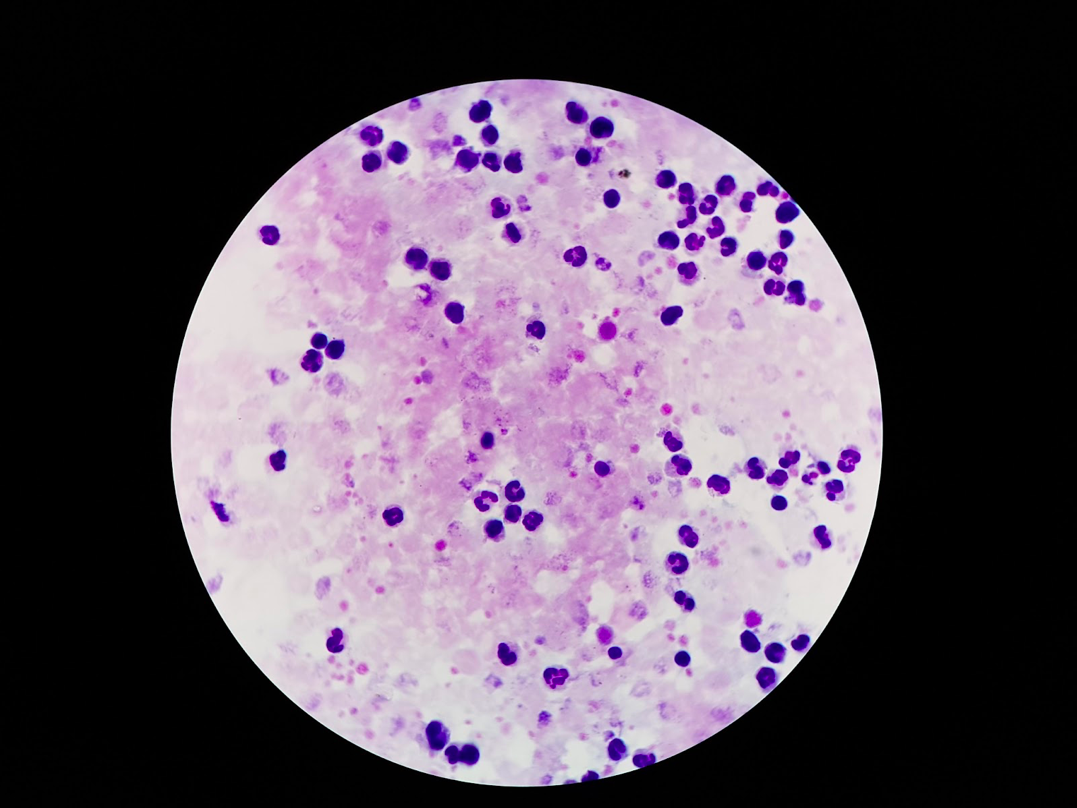
\includegraphics[width=0.4\linewidth]{./img/sample.png}} \hfill \subfloat[Imagem rotulada]{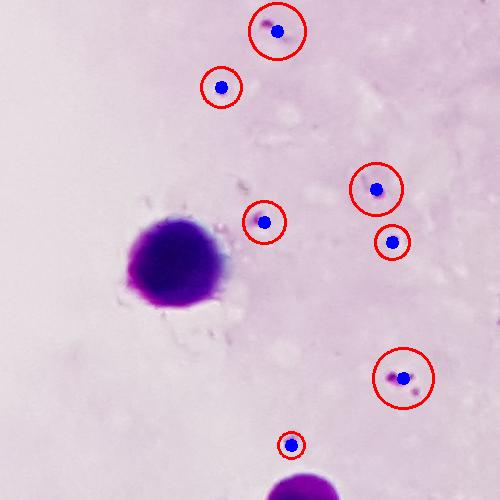
\includegraphics[width=0.35\linewidth]{./img/blood-circles.jpg}}\\
	\caption{Exemplos de imagens originais e recortadas contendo os rótulos da classe protozoário.} \label{img:dataset-samples}
\end{figure}
\end{frame}

\begin{frame}{Metodologia -- Distribuição das caixas delimitadoras}
\begin{figure}[H]
    \centering
    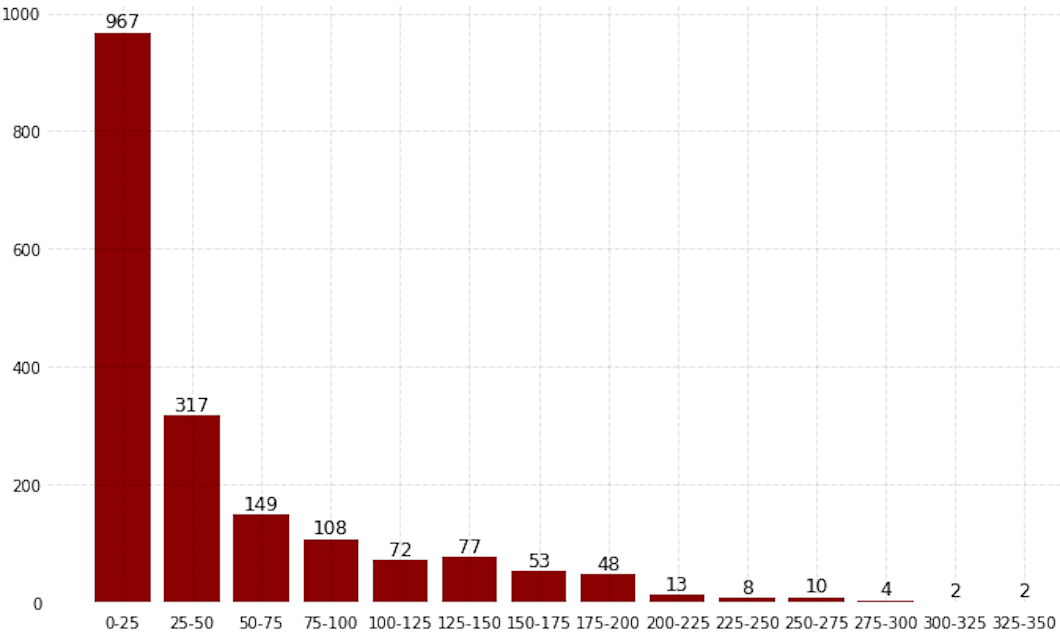
\includegraphics[width=0.65\linewidth]{./img/histogram.png}
    \caption{Histograma do número de caixas delimitadoras por imagem.}
    \label{fig:histogram}
\end{figure}
\end{frame}

\begin{frame}{Metodologia -- Regiões das caixas delimitadoras}
\begin{figure}[H]
    \centering
    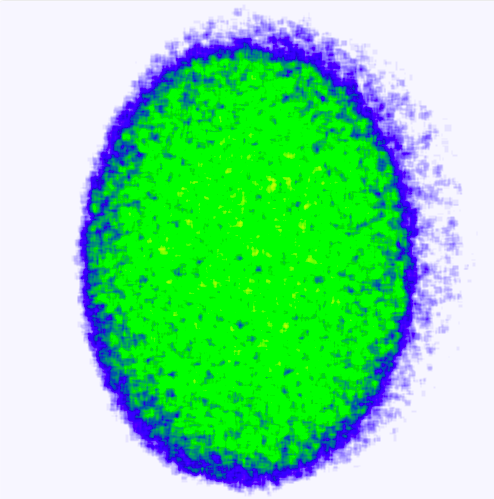
\includegraphics[width=0.5\textwidth,height=0.375\textwidth]{./img/heat-map.png}
    \caption{Mapa de calor da distribuição das caixas delimitadoras pela área da imagem.}
    \label{fig:heat-map}
\end{figure}
\end{frame}

\begin{frame}{Metodologia --  Validação e Avaliação}
\begin{itemize}
\item Validação Cruzada do tipo \alert{\emph{holdout}}
\begin{itemize}
    \item Treinamento: $70\%$
    \item Validação: $10\%$
    \item Teste: $20\%$
\end{itemize}
\ \ \newline
\item Regularização com o uso de \alert{\emph{early stopping}: $100$ épocas} na YOLOv5
\item \alert{Métricas}: Precisão, Revocação, $F_1$-\emph{Score} e mAP@0.5
\end{itemize}
\end{frame}

\begin{frame}{Metodologia -- Parâmetros e Hiperparâmetros}
\begin{itemize}
    \item \alert{YOLOv5} \emph{Nano}: $\num{1,7}$ milhões
    \item \alert{YOLOv5} \emph{Small}: $\num{7}$ milhões 
    \item \alert{YOLOv5} \emph{Medium}: ${20,8}$ milhões
    \ \ \newline
    \item \alert{YOLOv7} \emph{Tiny}: $\num{6}$ milhões
    \item \alert{YOLOv7} \emph{Standard}: $\num{36,4}$ milhões
    \item \alert{YOLOv7} \emph{Large}: $\num{70,7}$ milhões
    \ \ \newline
    \item Número de épocas: $300$ e $500$ épocas
    \item Taxa de aprendizado: $10^{-2}$
    \item Tamanho do \emph{batch}: $16$, $8$ e $4$
\end{itemize}
\end{frame}




\section{Resultados}
%!TEX root=../main.tex
\begin{frame}[shrink=8]{Resultados}
\begin{table}[h!]
\caption{Síntese dos resultados experimentais.} \label{tab:resultadosExperimentais}
\begin{footnotesize}
\begin{tabular}{cccccccc}
\toprule
\textbf{Modelo} & \textbf{Épocas} &\textbf{Precisão} & \textbf{Revocação} & \textbf{F-\emph{Score}} & \textbf{mAP@0.5} & \textbf{Parâmetros} & \textbf{Tempo}\\
\midrule
\textbf{YOLOv5 \emph{Medium}} & $300/300$ & $\SI{59,5}{\percent}$ & $\SI{63,1}{\percent}$ & $\SI{61,20}{\percent}$ & $\SI{55,5}{\percent}$ & $\num{20852934}$ & $\SI{9}{\hour}\SI{7}{\minute}$\\
\textbf{YOLOv5 Medium} & $264/500$ & $\SI{81,7}{\percent}$ & $\SI{78,9}{\percent}$ & $\SI{80,27}{\percent}$ & $\SI{79,9}{\percent}$ & $\num{20852934}$ & $\SI{9}{\hour}\SI{58}{\minute}$\\
\textbf{YOLOv5 Small} & $173/300$ & $\SI{81,5}{\percent}$ & $\SI{79,7}{\percent}$ & $\SI{80,58}{\percent}$ & $\SI{80,7}{\percent}$ & $\num{7012822}$ & $\SI{7}{\hour}\SI{26}{\minute}$\\
\textbf{YOLOv5 Small} & $194/500$ & $\SI{81,4}{\percent}$ & $\SI{79,4}{\percent}$ & $\SI{80,38}{\percent}$ & $\SI{80,4}{\percent}$ & $\num{7012822}$ & $\SI{6}{\hour}$\\
\textbf{YOLOv5 Nano} & $293/300$ & $\SI{79,5}{\percent}$ & $\SI{77,5}{\percent}$ & $\SI{78,48}{\percent}$ & $\SI{78,3}{\percent}$ & $\num{1760518}$ & $\SI{10}{\hour}\SI{19}{\minute}$\\
\textbf{YOLOv5 Nano} & $340/500$ & $\SI{79,9}{\percent}$ & $\SI{78,2}{\percent}$ & $\SI{79,04}{\percent}$ & $\SI{79,0}{\percent}$ & $\num{1760518}$ & $\SI{12}{\hour}\SI{38}{\minute}$\\
\midrule
\textbf{YOLOv7 Large} & $500/500$ & $\SI{80,6}{\percent}$ & $\SI{79,9}{\percent}$ & $\SI{80,24}{\percent}$ & $\SI{81,4}{\percent}$ & $\num{70782444}$ & $\SI{52}{\hour}\SI{5}{\minute}$\\
\textbf{YOLOv7 Standard} & $500/500$ & $\SI{79,2}{\percent}$ & $\SI{78,8}{\percent}$ & $\SI{78,99}{\percent}$ & $\SI{79,8}{\percent}$ & $\num{36481772}$ & $\SI{26}{\hour}\SI{34}{\minute}$\\
\textbf{YOLOv7 Tiny} & $500/500$ & $\SI{75,2}{\percent}$ & $\SI{77,9}{\percent}$ & $\SI{76,52}{\percent}$ & $\SI{77,0}{\percent}$ & $\num{6007596}$ & $\SI{23}{\hour}\SI{1}{\minute}$\\

\bottomrule
\end{tabular}
\end{footnotesize}
\end{table}
\end{frame}

\begin{frame}[shrink=8]{Resultados}
\begin{table}[h!]
\caption{Modelo melhor avaliado.} \label{tab:resultadosExperimentais}
\begin{footnotesize}
\begin{tabular}{cccccccc}
\toprule
\textbf{Modelo} & \textbf{Épocas} &\textbf{Precisão} & \textbf{Revocação} & \textbf{F-\emph{Score}} & \textbf{mAP@0.5} & \textbf{Parâmetros} & \textbf{Tempo}\\
\midrule
\textbf{YOLOv5 \emph{Medium}} & $300/300$ & $\SI{59,5}{\percent}$ & $\SI{63,1}{\percent}$ & $\SI{61,20}{\percent}$ & $\SI{55,5}{\percent}$ & $\num{20852934}$ & $\SI{9}{\hour}\SI{7}{\minute}$\\
\textbf{YOLOv5 Medium} & $264/500$ & $\SI{81,7}{\percent}$ & $\SI{78,9}{\percent}$ & $\SI{80,27}{\percent}$ & $\SI{79,9}{\percent}$ & $\num{20852934}$ & $\SI{9}{\hour}\SI{58}{\minute}$\\
\textbf{YOLOv5 Small} & $173/300$ & $\SI{81,5}{\percent}$ & $\SI{79,7}{\percent}$ & $\SI{80,58}{\percent}$ & $\SI{80,7}{\percent}$ & $\num{7012822}$ & $\SI{7}{\hour}\SI{26}{\minute}$\\
\textbf{YOLOv5 Small} & $194/500$ & $\SI{81,4}{\percent}$ & $\SI{79,4}{\percent}$ & $\SI{80,38}{\percent}$ & $\SI{80,4}{\percent}$ & $\num{7012822}$ & $\SI{6}{\hour}$\\
\textbf{YOLOv5 Nano} & $293/300$ & $\SI{79,5}{\percent}$ & $\SI{77,5}{\percent}$ & $\SI{78,48}{\percent}$ & $\SI{78,3}{\percent}$ & $\num{1760518}$ & $\SI{10}{\hour}\SI{19}{\minute}$\\
\textbf{YOLOv5 Nano} & $340/500$ & $\SI{79,9}{\percent}$ & $\SI{78,2}{\percent}$ & $\SI{79,04}{\percent}$ & $\SI{79,0}{\percent}$ & $\num{1760518}$ & $\SI{12}{\hour}\SI{38}{\minute}$\\
\midrule
\textcolor{blue}{\textbf{YOLOv7 Large}} & \textcolor{blue}{$500/500$} & \textcolor{blue}{$\SI{80,6}{\percent}$} & \textcolor{blue}{$\SI{79,9}{\percent}$} & \textcolor{blue}{$\SI{80,24}{\percent}$} & \textcolor{blue}{$\SI{81,4}{\percent}$} & \textcolor{blue}{$\num{70782444}$} & \textcolor{blue}{$\SI{52}{\hour}\SI{5}{\minute}$}\\
\textbf{YOLOv7 Standard} & $500/500$ & $\SI{79,2}{\percent}$ & $\SI{78,8}{\percent}$ & $\SI{78,99}{\percent}$ & $\SI{79,8}{\percent}$ & $\num{36481772}$ & $\SI{26}{\hour}\SI{34}{\minute}$\\
\textbf{YOLOv7 Tiny} & $500/500$ & $\SI{75,2}{\percent}$ & $\SI{77,9}{\percent}$ & $\SI{76,52}{\percent}$ & $\SI{77,0}{\percent}$ & $\num{6007596}$ & $\SI{23}{\hour}\SI{1}{\minute}$\\
\bottomrule
\end{tabular}
\end{footnotesize}
\end{table}
\end{frame}

\begin{frame}[shrink=8]{Resultados}
\begin{table}[h!]
\caption{Modelo com as menores métricas de desempenho.} \label{tab:resultadosExperimentais}
\begin{footnotesize}
\begin{tabular}{cccccccc}
\toprule
\textbf{Modelo} & \textbf{Épocas} &\textbf{Precisão} & \textbf{Revocação} & \textbf{F-\emph{Score}} & \textbf{mAP@0.5} & \textbf{Parâmetros} & \textbf{Tempo}\\
\midrule
\textcolor{blue}{\textbf{YOLOv5 \emph{Medium}}} & \textcolor{blue}{$300/300$} & \textcolor{blue}{$\SI{59,5}{\percent}$} & \textcolor{blue}{$\SI{63,1}{\percent}$} & \textcolor{blue}{$\SI{61,20}{\percent}$} & \textcolor{blue}{$\SI{55,5}{\percent}$} & \textcolor{blue}{$\num{20852934}$} & \textcolor{blue}{$\SI{9}{\hour}\SI{7}{\minute}$}\\
\textbf{YOLOv5 Medium} & $264/500$ & $\SI{81,7}{\percent}$ & $\SI{78,9}{\percent}$ & $\SI{80,27}{\percent}$ & $\SI{79,9}{\percent}$ & $\num{20852934}$ & $\SI{9}{\hour}\SI{58}{\minute}$\\
\textbf{YOLOv5 Small} & $173/300$ & $\SI{81,5}{\percent}$ & $\SI{79,7}{\percent}$ & $\SI{80,58}{\percent}$ & $\SI{80,7}{\percent}$ & $\num{7012822}$ & $\SI{7}{\hour}\SI{26}{\minute}$\\
\textbf{YOLOv5 Small} & $194/500$ & $\SI{81,4}{\percent}$ & $\SI{79,4}{\percent}$ & $\SI{80,38}{\percent}$ & $\SI{80,4}{\percent}$ & $\num{7012822}$ & $\SI{6}{\hour}$\\
\textbf{YOLOv5 Nano} & $293/300$ & $\SI{79,5}{\percent}$ & $\SI{77,5}{\percent}$ & $\SI{78,48}{\percent}$ & $\SI{78,3}{\percent}$ & $\num{1760518}$ & $\SI{10}{\hour}\SI{19}{\minute}$\\
\textbf{YOLOv5 Nano} & $340/500$ & $\SI{79,9}{\percent}$ & $\SI{78,2}{\percent}$ & $\SI{79,04}{\percent}$ & $\SI{79,0}{\percent}$ & $\num{1760518}$ & $\SI{12}{\hour}\SI{38}{\minute}$\\
\midrule
\textbf{YOLOv7 Large} & $500/500$ & $\SI{80,6}{\percent}$ & $\SI{79,9}{\percent}$ & $\SI{80,24}{\percent}$ & $\SI{81,4}{\percent}$ & $\num{70782444}$ & $\SI{52}{\hour}\SI{5}{\minute}$\\
\textbf{YOLOv7 Standard} & $500/500$ & $\SI{79,2}{\percent}$ & $\SI{78,8}{\percent}$ & $\SI{78,99}{\percent}$ & $\SI{79,8}{\percent}$ & $\num{36481772}$ & $\SI{26}{\hour}\SI{34}{\minute}$\\
\textbf{YOLOv7 Tiny} & $500/500$ & $\SI{75,2}{\percent}$ & $\SI{77,9}{\percent}$ & $\SI{76,52}{\percent}$ & $\SI{77,0}{\percent}$ & $\num{6007596}$ & $\SI{23}{\hour}\SI{1}{\minute}$\\
\bottomrule
\end{tabular}
\end{footnotesize}
\end{table}
\end{frame}

\begin{frame}[shrink=8]{Resultados}
\begin{table}[h!]
\caption{Modelo mais leve melhor avaliado.} \label{tab:resultadosExperimentais}
\begin{footnotesize}
\begin{tabular}{cccccccc}
\toprule
\textbf{Modelo} & \textbf{Épocas} &\textbf{Precisão} & \textbf{Revocação} & \textbf{F-\emph{Score}} & \textbf{mAP@0.5} & \textbf{Parâmetros} & \textbf{Tempo}\\
\midrule
\textbf{YOLOv5 \emph{Medium}} & $300/300$ & $\SI{59,5}{\percent}$ & $\SI{63,1}{\percent}$ & $\SI{61,20}{\percent}$ & $\SI{55,5}{\percent}$ & $\num{20852934}$ & $\SI{9}{\hour}\SI{7}{\minute}$\\
\textbf{YOLOv5 Medium} & $264/500$ & $\SI{81,7}{\percent}$ & $\SI{78,9}{\percent}$ & $\SI{80,27}{\percent}$ & $\SI{79,9}{\percent}$ & $\num{20852934}$ & $\SI{9}{\hour}\SI{58}{\minute}$\\
\textbf{YOLOv5 Small} & $173/300$ & $\SI{81,5}{\percent}$ & $\SI{79,7}{\percent}$ & $\SI{80,58}{\percent}$ & $\SI{80,7}{\percent}$ & $\num{7012822}$ & $\SI{7}{\hour}\SI{26}{\minute}$\\
\textbf{YOLOv5 Small} & $194/500$ & $\SI{81,4}{\percent}$ & $\SI{79,4}{\percent}$ & $\SI{80,38}{\percent}$ & $\SI{80,4}{\percent}$ & $\num{7012822}$ & $\SI{6}{\hour}$\\
\textbf{YOLOv5 Nano} & $293/300$ & $\SI{79,5}{\percent}$ & $\SI{77,5}{\percent}$ & $\SI{78,48}{\percent}$ & $\SI{78,3}{\percent}$ & $\num{1760518}$ & $\SI{10}{\hour}\SI{19}{\minute}$\\
\textcolor{blue}{\textbf{YOLOv5 Nano}} & \textcolor{blue}{$340/500$} & \textcolor{blue}{$\SI{79,9}{\percent}$} & \textcolor{blue}{$\SI{78,2}{\percent}$} & \textcolor{blue}{$\SI{79,04}{\percent}$} & \textcolor{blue}{$\SI{79,0}{\percent}$} & \textcolor{blue}{$\num{1760518}$} & \textcolor{blue}{$\SI{12}{\hour}\SI{38}{\minute}$}\\
\midrule
\textbf{YOLOv7 Large} & $500/500$ & $\SI{80,6}{\percent}$ & $\SI{79,9}{\percent}$ & $\SI{80,24}{\percent}$ & $\SI{81,4}{\percent}$ & $\num{70782444}$ & $\SI{52}{\hour}\SI{5}{\minute}$\\
\textbf{YOLOv7 Standard} & $500/500$ & $\SI{79,2}{\percent}$ & $\SI{78,8}{\percent}$ & $\SI{78,99}{\percent}$ & $\SI{79,8}{\percent}$ & $\num{36481772}$ & $\SI{26}{\hour}\SI{34}{\minute}$\\
\textbf{YOLOv7 Tiny} & $500/500$ & $\SI{75,2}{\percent}$ & $\SI{77,9}{\percent}$ & $\SI{76,52}{\percent}$ & $\SI{77,0}{\percent}$ & $\num{6007596}$ & $\SI{23}{\hour}\SI{1}{\minute}$\\
\bottomrule
\end{tabular}
\end{footnotesize}
\end{table}
\end{frame}

\begin{frame}{Resultados}
    \begin{figure}[H]
	\centering
	\subfloat[Desejado]{ 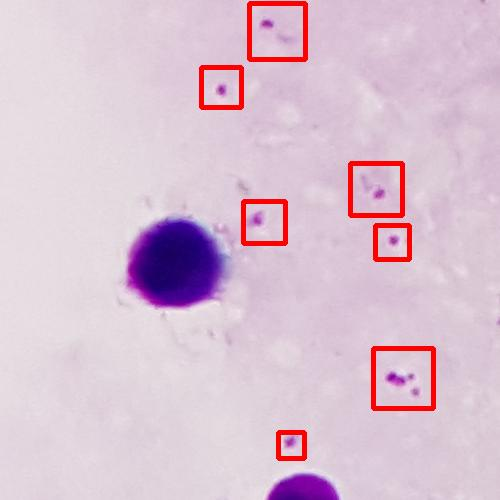
\includegraphics[width=0.35\linewidth]{./img/results/result.jpg}}
	%\hfill
	\subfloat[Previsto]{    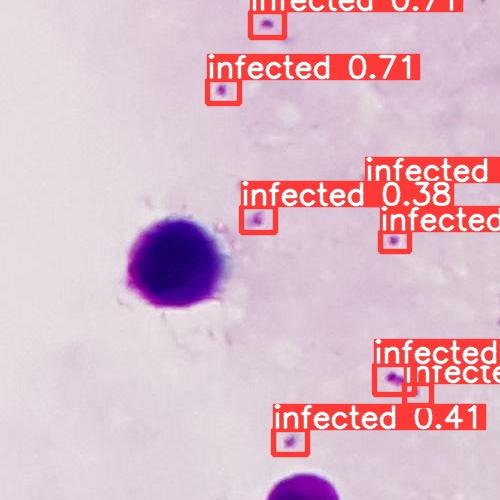
\includegraphics[width=0.35\linewidth]{./img/results/predicted.jpg}} \\
	\caption{Resultados desejados e inferidos pelo modelo YOLOv5.} \label{img:yolov5}
\end{figure}
\end{frame}

\begin{frame}
    \begin{figure}[H]
	\centering
	%\hfill
    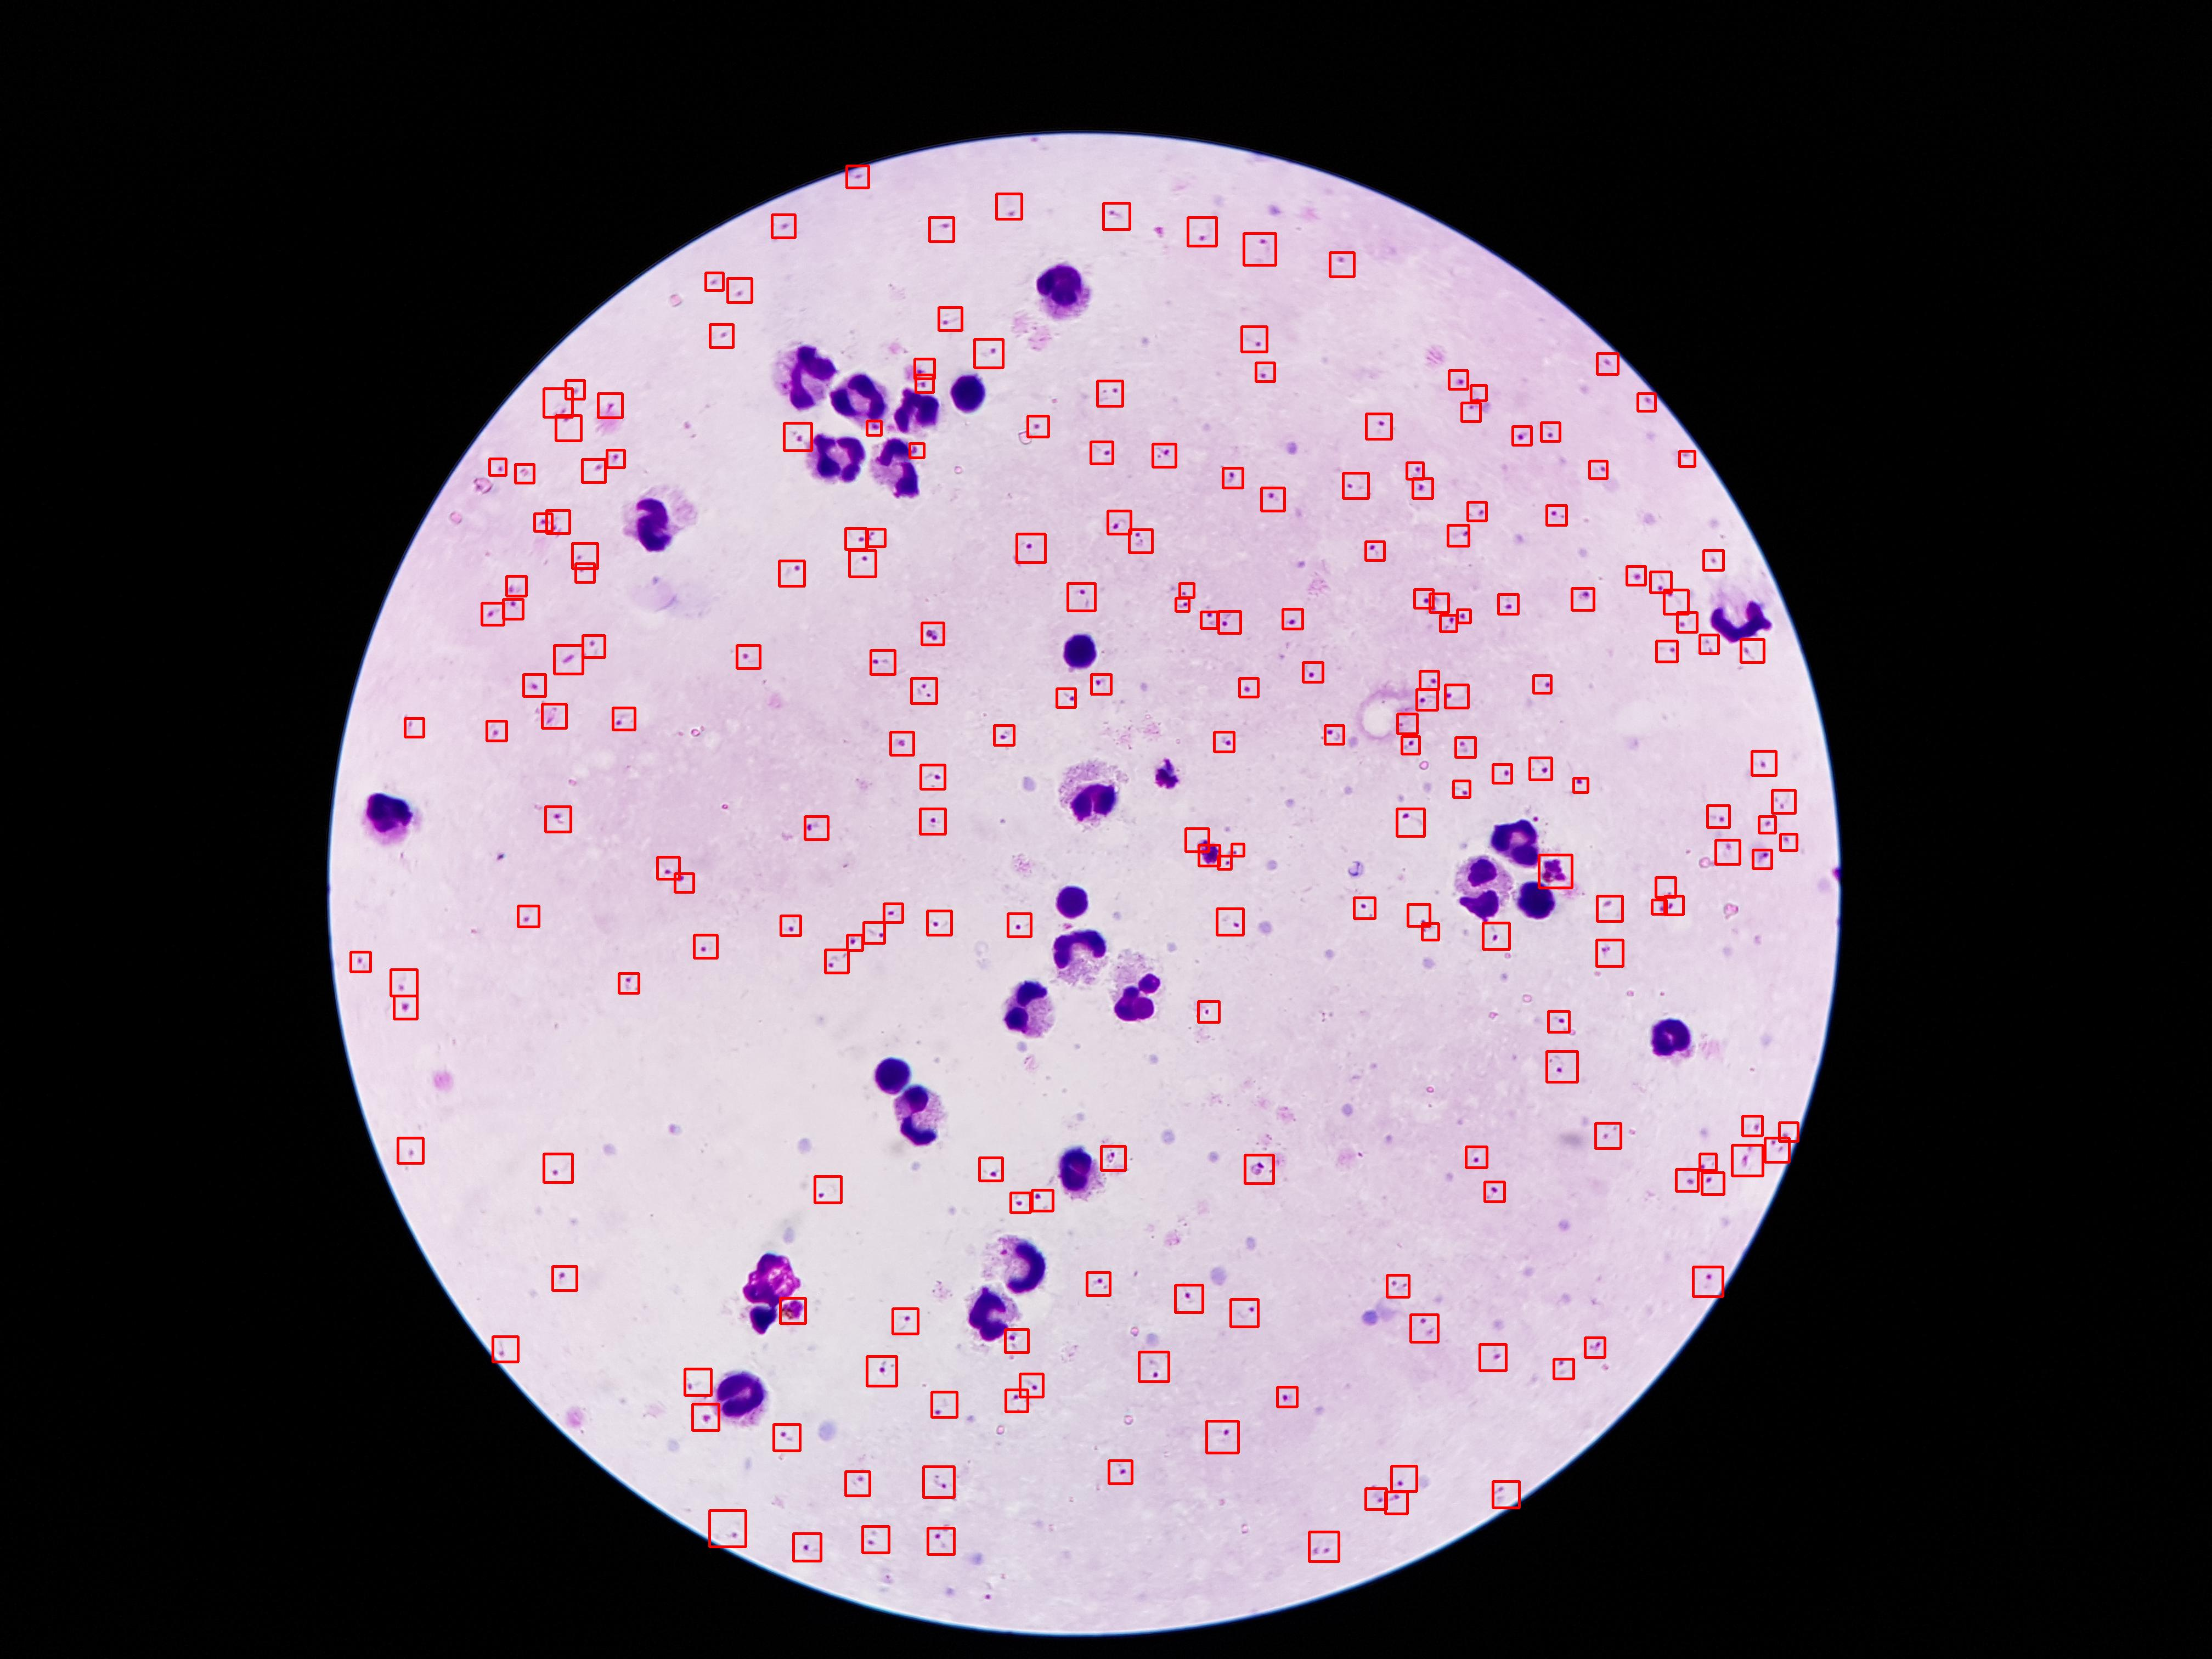
\includegraphics[width=0.73\linewidth]{./img/results/result5-v7-ideal.jpg} \\
	\caption{Predição ideal da imagem.} \label{img:yolov7-ideal}
\end{figure}
\end{frame}

\begin{frame}
    \begin{figure}[H]
	\centering
	%\hfill
    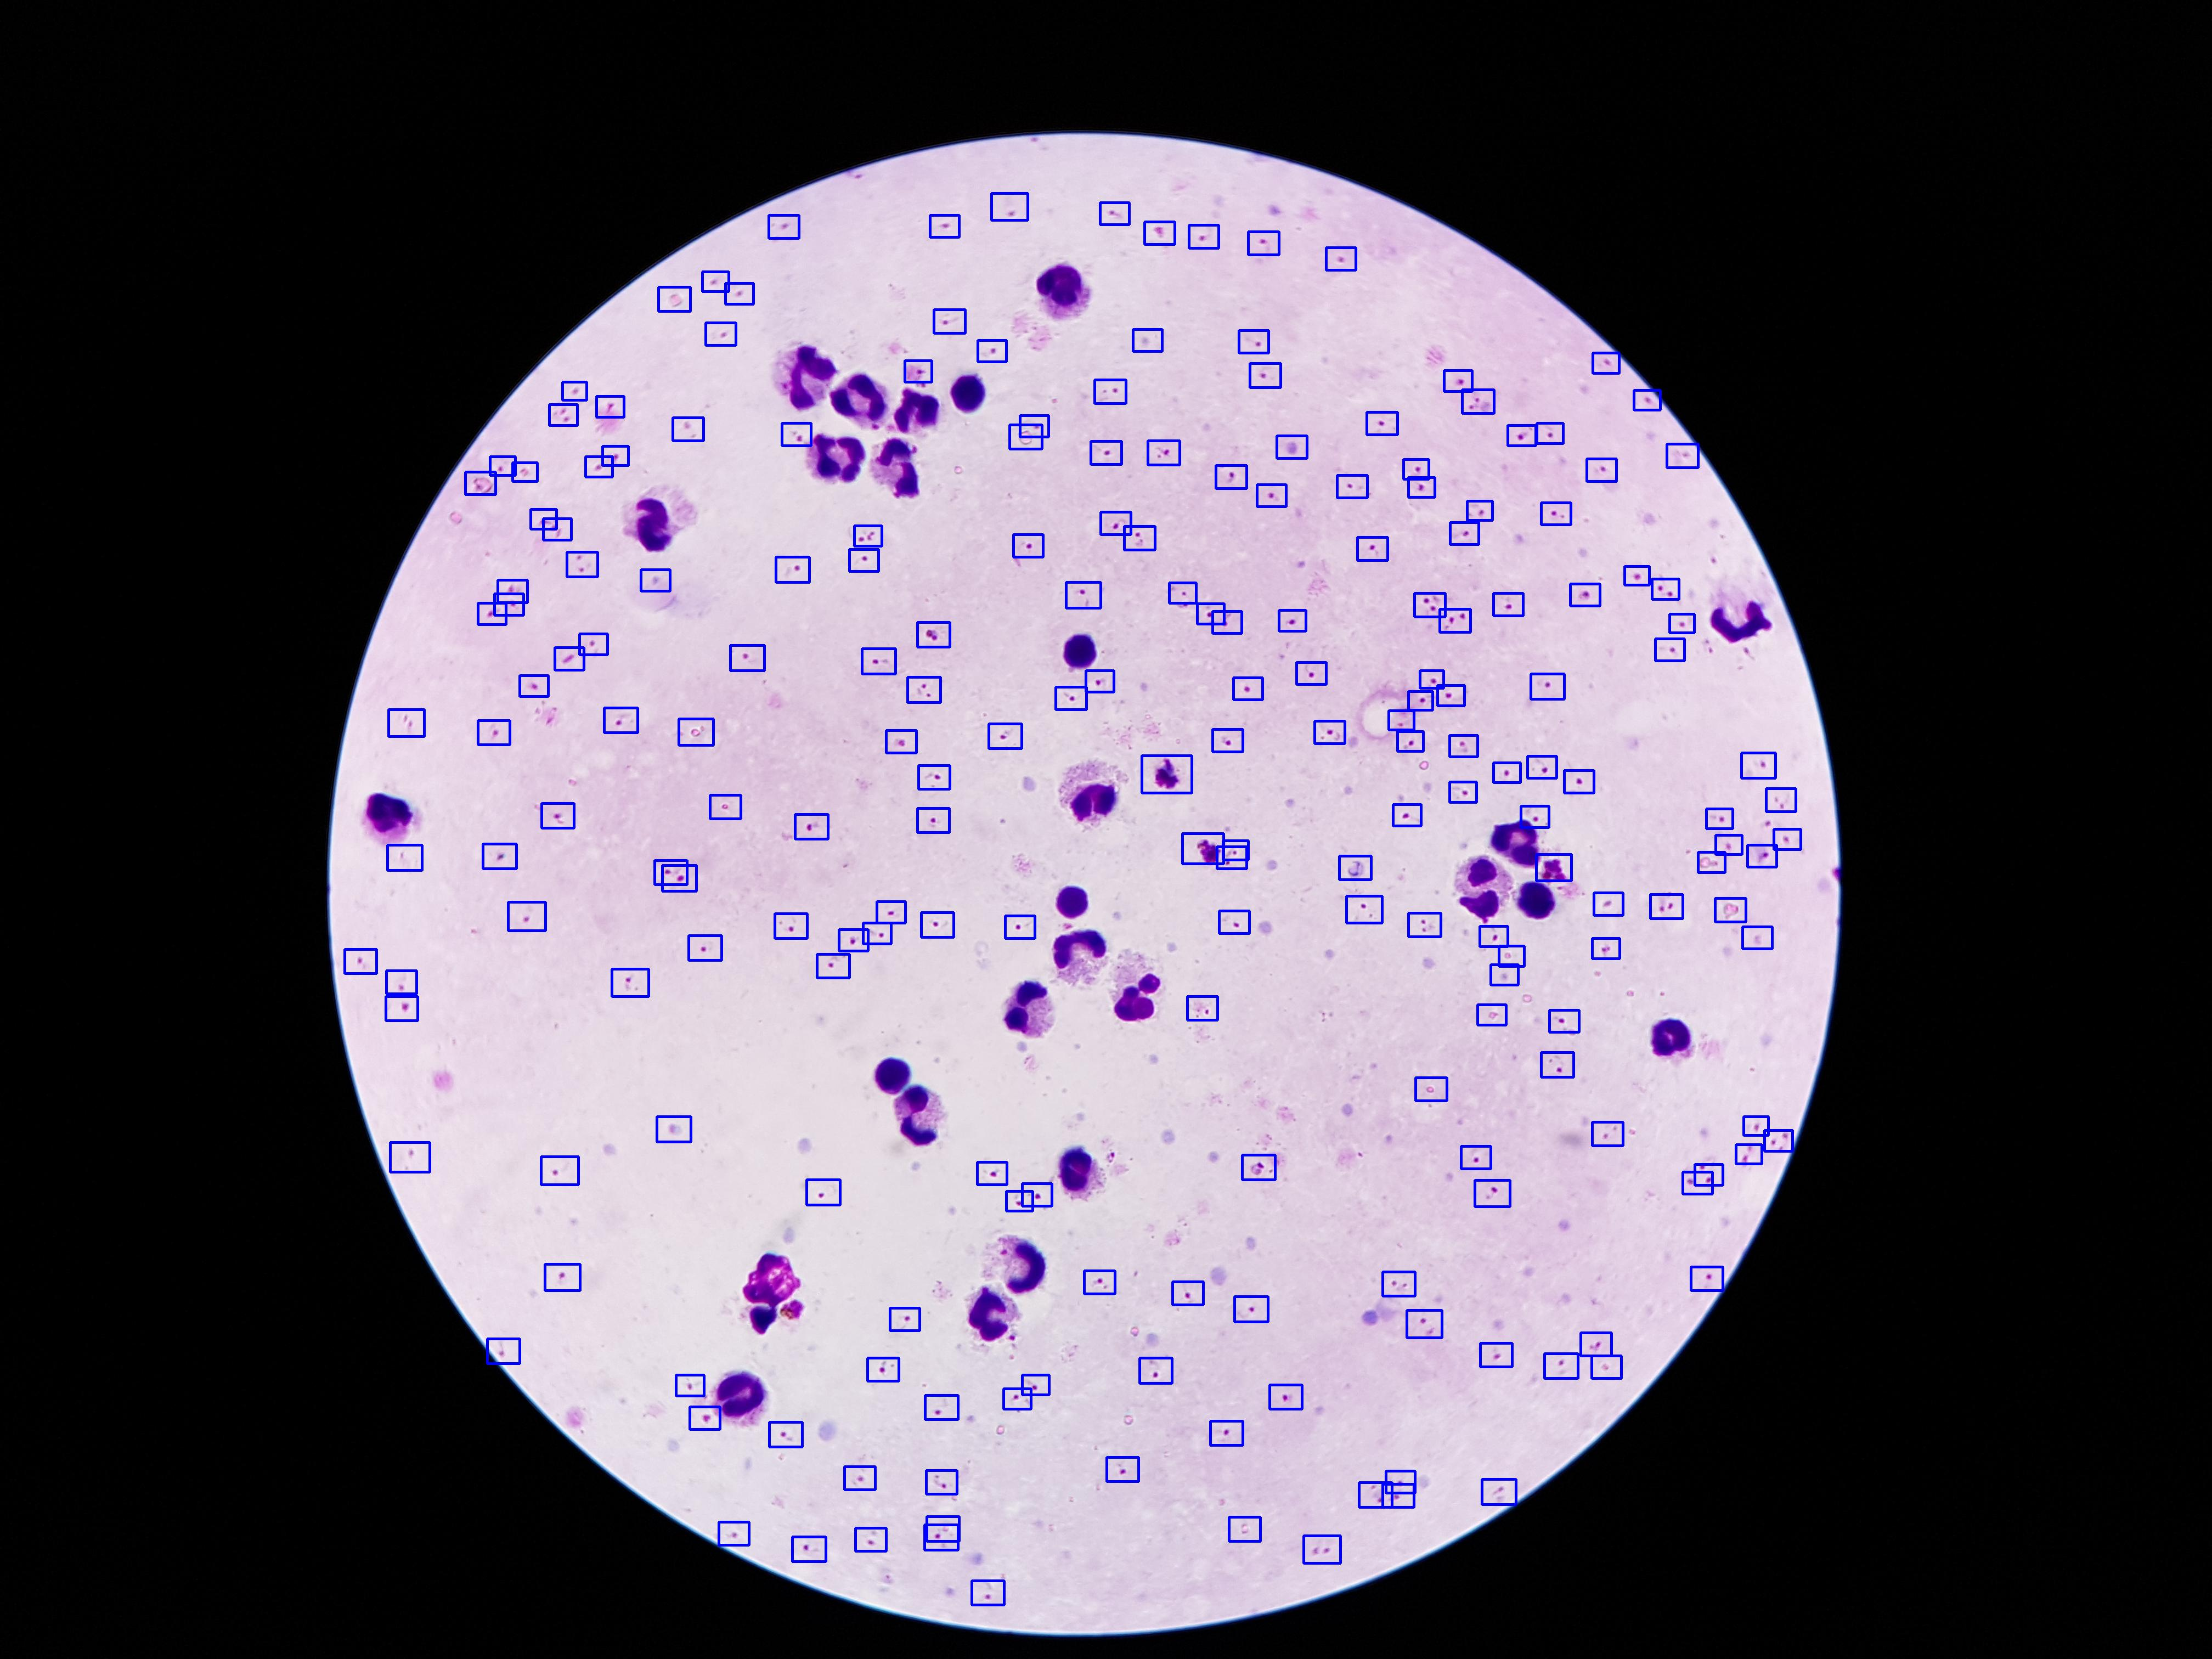
\includegraphics[width=0.73\linewidth]{./img/results/result5-v7-detected.jpg} \\
	\caption{Detecção pelo modelo YOLOv7.} \label{img:yolov7-detected}
\end{figure}
\end{frame}

\begin{frame}
    \begin{figure}[H]
	\centering
	%\hfill
    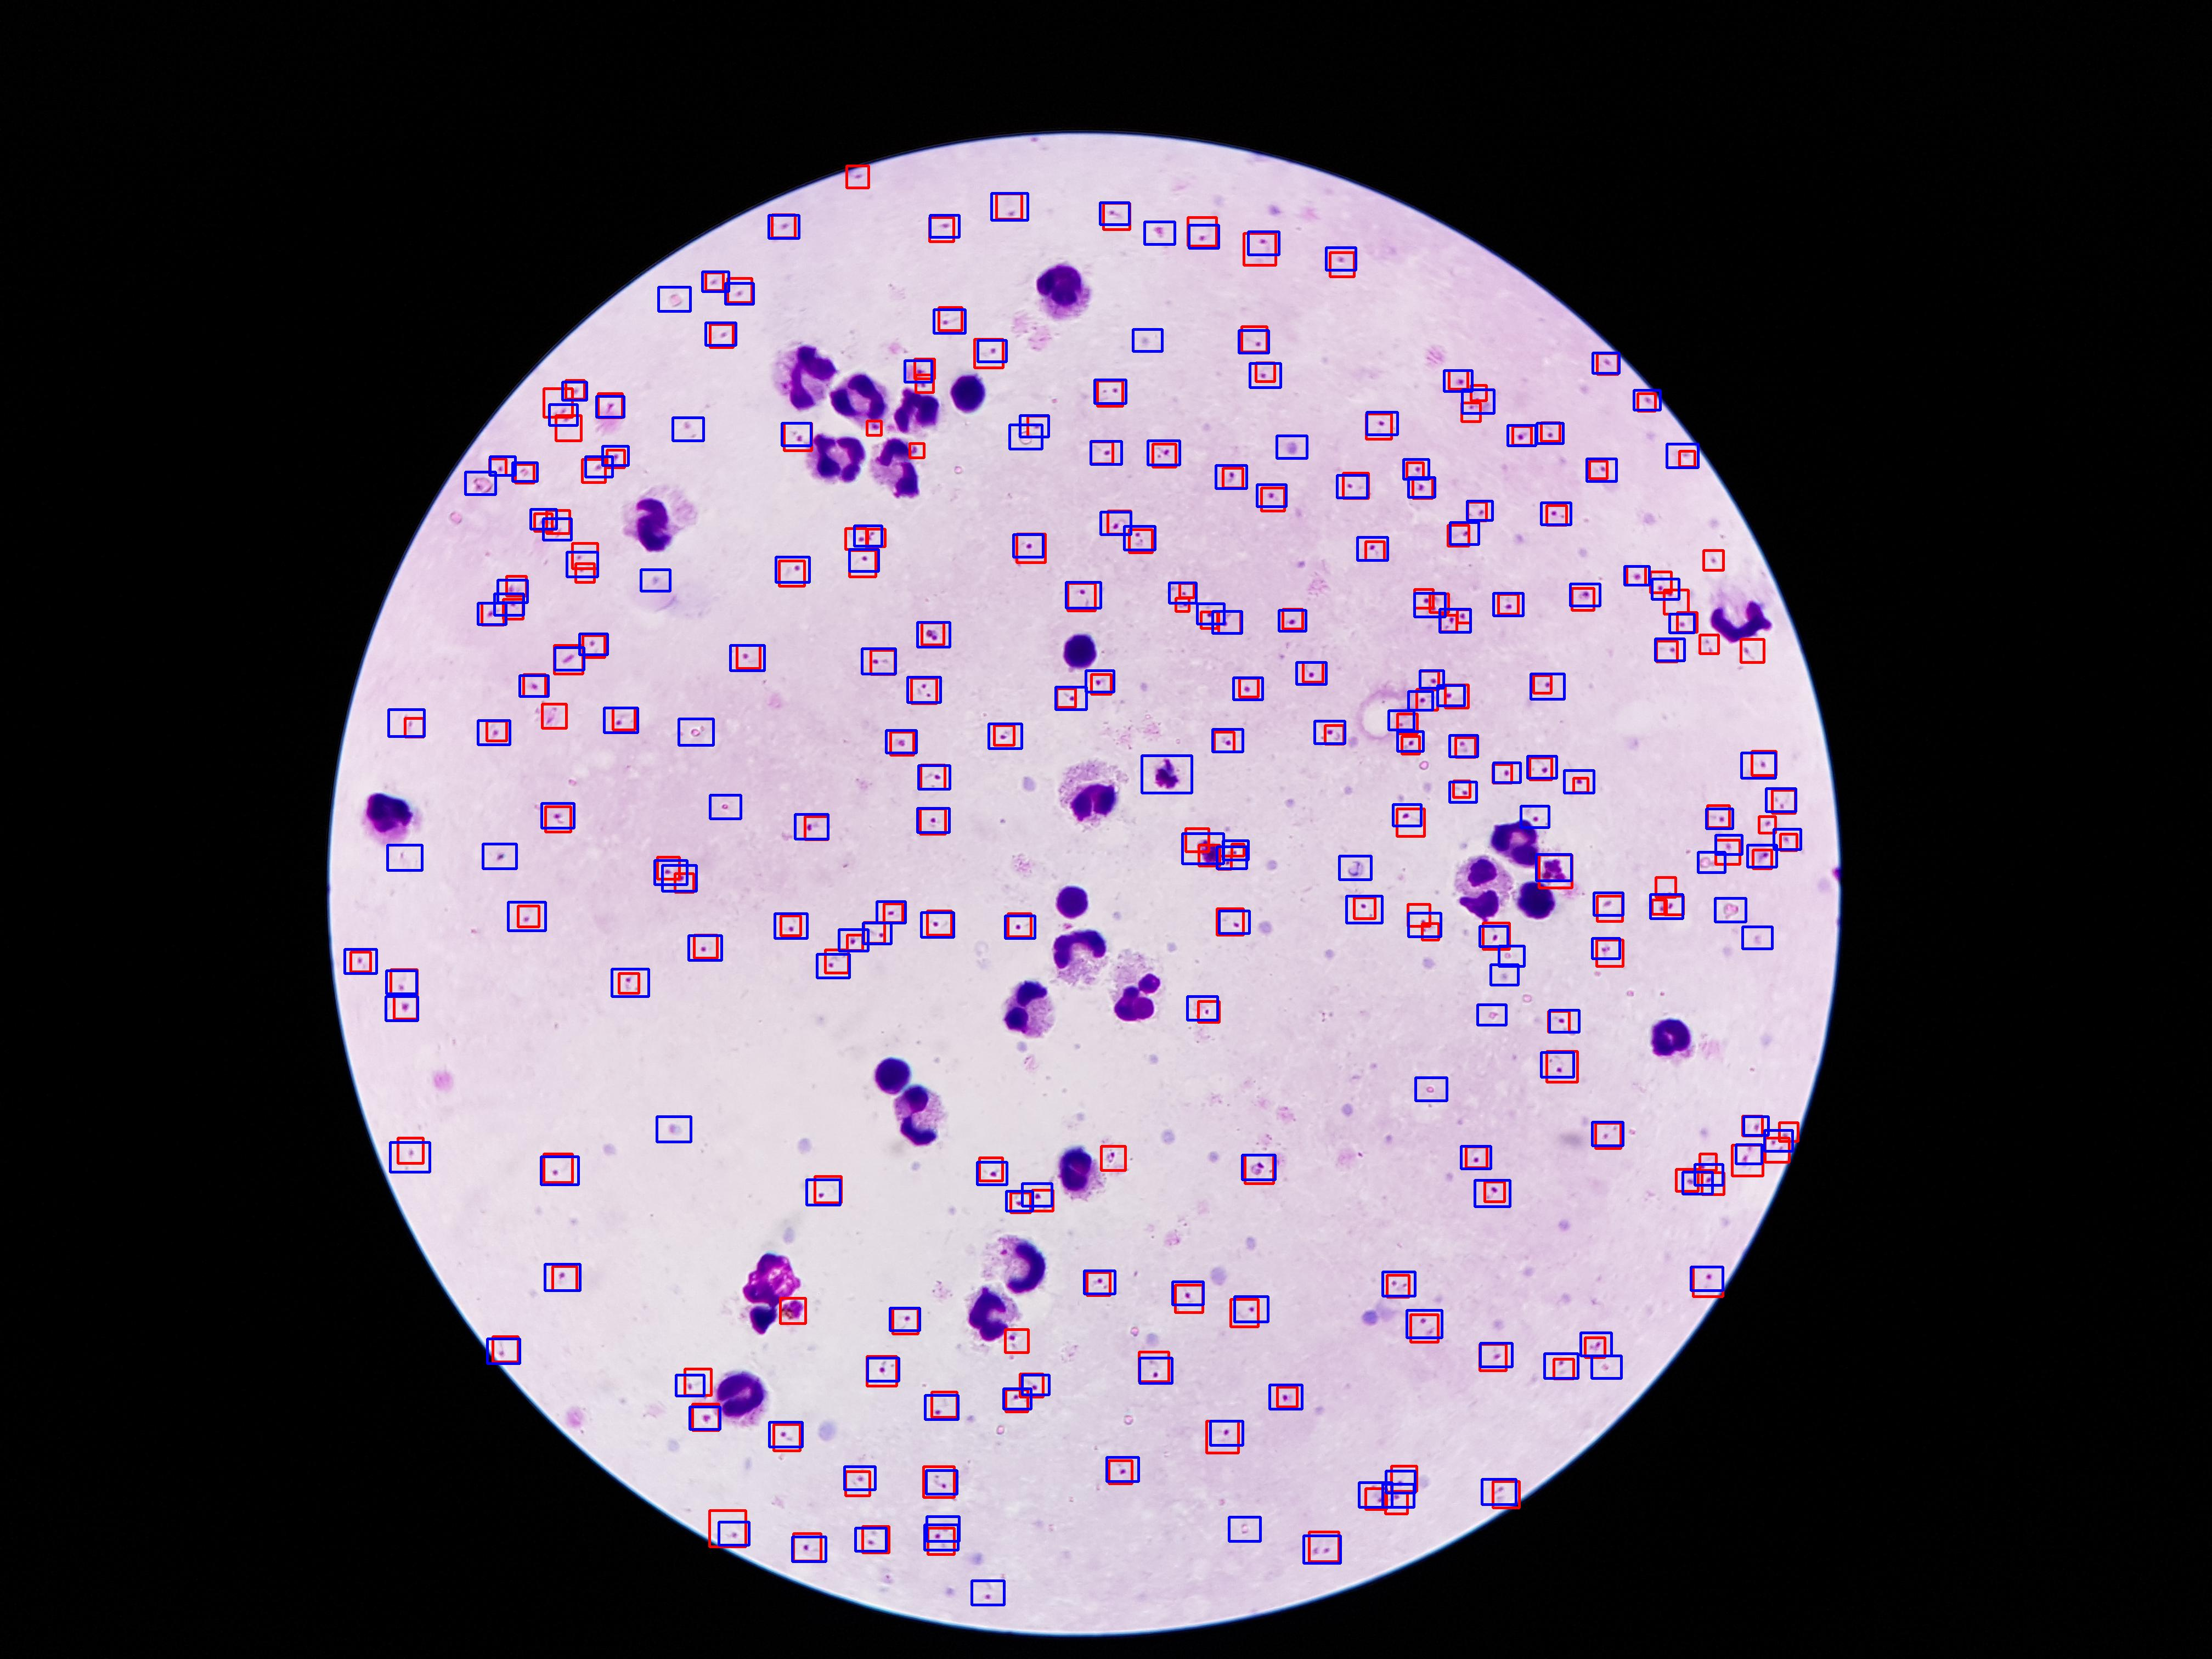
\includegraphics[width=0.73\linewidth]{./img/results/result5-v7.jpg} \\
	\caption{Comparação entre o resultado ideal e o detectado do modelo YOLOv7.} \label{img:yolov7}
\end{figure}
\end{frame}




%\section{Estudo de Caso em Pavimentações no Brasil}
%%!TEX root=../main.tex
\begin{frame}{Estudo de Caso: Pavimentações no Brasil}
    \begin{block}{Questão Motriz}
    Como o melhor modelo identificado se comporta em um cenário brasileiro?
    \end{block}
    \pause
    \begin{itemize}
    \item \emph{Road Traversing Knowledge} -- \alert{RTK \emph{dataset}} \cite{Rateke2019}
    \item Anotado originalmente para segmentação
    \item Imagens com dimensões $352 \times 288$ \emph{pixels}
    \end{itemize}
\end{frame}

\begin{frame}{Estudo de Caso: RTK \emph{dataset}}
   \begin{table}[h!]
\begin{center}
\caption{Descrição estatística do pré-processamento do RTK \emph{dataset}.} \label{tab:boundingboxes}
\begin{footnotesize}
\begin{tabular}{cccccccccc}
\toprule
        & \multicolumn{3}{c}{\textbf{Comprimento}} & & \multicolumn{3}{c}{\textbf{Largura}} & & \textbf{Exemplos} \\
        \cmidrule{2-4} \cmidrule{6-8} \cmidrule{10-10}
      &  \textbf{Média} & \textbf{Máx} & \textbf{Mín} & &    \textbf{Média} & \textbf{Máx} & \textbf{Mín} & & \textbf{Quantidade}\\
\midrule
\textbf{Classe D00} & $43.27 \pm 26.06$ & 98 & 6 & & $33.61 \pm 21.17$ & 87 & 3 & & 36\\
\textbf{Classe D10} & $18.76 \pm 21.00$ & 107 & 2 & & $42.24 \pm 47.70$ & 345 & 5 & & 390\\
\textbf{Classe D40} & $13.92 \pm 10.11$ & 62 & 3 & & $34.52 \pm 17.38$ & 93 & 4 & & 105\\
\bottomrule
\end{tabular}
\end{footnotesize}
\end{center}
\end{table}
\end{frame}


\begin{frame}{Estudo de Caso: Exemplos}
    \begin{figure}[h!]
    	\centering
    	\hfill {\includegraphics[width=0.32\linewidth]{./img/cracks_1.jpg}}
    	\subfloat{\includegraphics[width=0.32\linewidth]{./img/cracks_2.jpg}}
    	\subfloat{\includegraphics[width=0.32\linewidth]{./img/pothole_6.jpg}}
    	\caption{Exemplos do RTK \emph{dataset} com rótulos de classes mapeados.} \label{img:rtk}
    \end{figure}
\end{frame}

\begin{frame}{Estudo de Caso: Metodologia}
\begin{itemize}
    \item Transferência de aprendizado utilizando a arquitetura YOLOv5 com a Configuração 4
    \item Validação cruzada \emph{holdout}
    \begin{itemize}
    \item Treinamento: $70\%$
    \item Validação: $10\%$
    \item Teste: $20\%$
\end{itemize}
\ \ \newline
\item Regularização com o uso de \alert{\emph{early stopping}}
\item \alert{Métricas}: Precisão, Revocação, $F_1$-\emph{Score} e mAP
\end{itemize}
\end{frame}


\begin{frame}{Estudo de Caso: Resultados}
\begin{table}[h!]
\begin{center}
\caption{Desempenho da rede na previsão de falhas em pavimentações asfálticas no Brasil.} \label{tab:yoloBrasil}
\begin{tabular}{ccccc}
	\toprule
	  & \textbf{Precisão} & \textbf{Revocação} & $\mathbf{F_1}$\textbf{-Score} & \textbf{mAP}$\mathbf{@0.5}$\\
	\midrule
\textbf{Todas as Classes} & \SI{43,8}{\percent} & \SI{51,0}{\percent} & \SI{47,1}{\percent} & \SI{45,6}{\percent}\\
\textbf{Classe D00} & \SI{18,7}{\percent} & \SI{23,4}{\percent} & \SI{20,8}{\percent} & \SI{11,5}{\percent}\\
\textbf{Classe D10} & \SI{42,6}{\percent} & \SI{45,0}{\percent} & \SI{43,8}{\percent} & \SI{40,9}{\percent}\\
\textbf{Classe D40} & \SI{70,2}{\percent} & \SI{84,6}{\percent} & \SI{76,7}{\percent} & \SI{84,3}{\percent}\\
\bottomrule
\end{tabular}
\end{center}
\end{table}

\end{frame}

\begin{frame}{Estudo de Caso: Resultados}
\begin{figure}[h!]
	\centering
	\hfill \subfloat[Exemplo 1 -- Desejado]{\includegraphics[width=0.45\linewidth]{./img/pothole_6.jpg}} 	\hfill
	\subfloat[Exemplo 1 -- Previsto]{\includegraphics[width=0.45\linewidth]{./img/detected_6.jpg}} \hfill
    \caption{Exemplos de previsão do modelo no cenário brasileiro.}
\end{figure}
\end{frame}

\begin{frame}{Estudo de Caso: Resultados}
\begin{figure}[h!]
	\centering
	\hfill\subfloat[Exemplo 2 -- Desejado]
	{\includegraphics[width=0.45\linewidth]{./img/pothole_5.jpg}}\hfill
	\subfloat[Exemplo 2 -- Previsto]
	{\includegraphics[width=0.45\linewidth]{./img/detected_5.jpg}}\hfill
	\caption{Exemplos de previsão do modelo no cenário brasileiro.}
	
\end{figure}
\end{frame}

\begin{frame}{Estudo de Caso: Análise dos Resultados}
\begin{itemize}
    \item Transferência Negativa de Aprendizado: decréscimo percentual do mAP@0.5 de $\SI{14,25}{\percent}$
    \ \ \newline
    \item Tamanho das \emph{bounding boxes}, resolução das imagens, distância entre domínio de origem e de aplicação, etc.
    \ \ \newline
    \item Necessidade de elaborar bases de dados representativas para o Brasil
\end{itemize}

\end{frame}


\section{Considerações Finais}
%!TEX root=../main.tex
\begin{frame}{Considerações Finais}
    \begin{itemize}
          \item A solução baseada em YOLO e desenvolvida neste trabalho é um modelo satisfatório para a tarefa de detecção de protozoários responsáveis pela malária
          \ \ \newline
          \item Identificação de configuração da YOLOv7 com melhor desempenho
          \begin{itemize}
              \item \emph{Large} para $500$ épocas
              \item \mbox{$\textrm{mAP@0.5} = \SI{81,4}{\percent}$} 
          \end{itemize}
          \ \ \newline
          \item As entradas para o modelo foram imagens microscópicas originais, sem processamento prévio das mesmas
    \end{itemize}
\end{frame}

\begin{frame}{Considerações Finais: Próximos Passos}
     \begin{itemize}
            \item Melhorar o desempenho da solução, buscando explorar também as novas arquiteturas, suas configurações e ajuste fino de parâmetros
            \ \ \newline
            \item As imagens poderão ser divididas e as caixas delimitadoras alteradas, focando melhorar o desempenho dos treinos e testes com as novas versões.
        \end{itemize}
\end{frame}


\begin{frame}[allowframebreaks] {Referências}
\bibliographystyle{sbc}
\bibliography{ref}
\end{frame}


\institute{\small{Laboratório de Sistemas Inteligentes\\
Escola Superior de Tecnologia\\
Universidade do Estado do Amazonas}
}

{
\setbeamertemplate{footline}{}
\frame{\titlepage}
}

\end{document}
